\chapter{Silence}

\section{Signal}

\keywords{relation with our surroundings}

\noindent Two of us are walking down a path leading to the entrance of
the monastery. We are talking about one thing or another, but as we
enter, we notice the silence and our conversation stops. The Dhamma hall
is through the next door, and we don't want to disturb anyone who might
be meditating inside. We close the door quietly behind us. We are headed
somewhere else in the building, but the significance of the Dhamma Hall
is greater than that mundane task.

The silence of listening creates an implied relation with our
surroundings. In the earlier case, with the person who might be sitting
in the Dhamma Hall. But even if we could have seen that there was nobody
inside, we would still lower our voices or stay silent. When we enter,
the silence serves as a signal to pay attention. We give space for the
values beyond ourselves represented by the Dhamma Hall being, as it is,
dedicated to the truths of the heart and mind.

\enlargethispage*{\baselineskip}

In this context, silence is a signal which directs us to remember that
which is beyond the worldly values. When we enter a church, monastery or
other sacred space, we look beyond the noisy, worldly affairs and beyond
our usual preoccupation with ourselves.

We have enough experience of noisy chatter to know that profound
comprehension is not found there. So we fall silent to give attention to
listening, to be a part of the understanding which we cannot express in
words. We move in silence, we listen in silence. We carefully keep
ourselves out of the way, so that we can hear the message of the place
and let the activity speak for itself. This silence is a presence which
is not isolating, but is rather inclusive of the space and the other
beings who live there. In the words of David Whyte,\footnote{\href{https://www.goodreads.com/quotes/10119971-the-winter-of-listening-no-one-but-me-by-the}{The
  Winter of Listening by David Whyte}}

\begin{quote}
You can belong\\
to everything\\
simply by listening.
\end{quote}

\section{Valuable}

\keywords{value of silence, serenity in silence}

\noindent Silence also expresses how much we value what we are doing.
Being silent and maintaining attention is an expression of alertness and
shows respect for the current activity. This is both an inward and
outward signal. Others see that whatever we are doing, it requires
silence. And we too witness ourselves being silent, when we voluntarily
restrain our impact on ourselves and on our surroundings. This
communicates that where we are and what we are doing is more significant
than chattering about ourselves.

Calmness, understanding and silence are closely connected. We stop
speaking and pay careful attention to investigate and understand
phenomena. After this verbal silence, the mind continues, `Why? Why?'
But when the penny drops, when there is that `Aha!' moment, the mind
stops chattering and we are silent, grateful for the understanding. In
that content and serene mood, we stay silent. For the moment, nothing
further is required.

\begin{quote}
On hearing true teachings\\
the hearts of those who are receptive\\
become serene,\\
like a lake, deep, clear and still.

\bigskip

\quoteRef{%

Dhp 82.\footnote{\href{https://forestsangha.org/teachings/books/a-dhammapada-for-contemplation?language=English}{A
  Dhammapada for Contemplation by Ajahn Munindo (forestsangha.org)}}

}
\end{quote}

\section{Lying down meditation method}

\noindent Physical stillness is most characteristic in the lying down
meditation posture. In this posture the muscles of the body are
completely relaxed. Although this creates a sense of ease and comfort,
one has to take care to avoid falling asleep. When you are physically
tired, this posture is not recommended for formal meditation. Rather,
sitting, walking or standing meditation are preferable as they raise the
body's level of alertness through the physical effort.

\clearpage
\thispagestyle{empty}\mbox{}
\contentFullBleed{%
\centering
\null\vfill

\hspace*{20mm}%
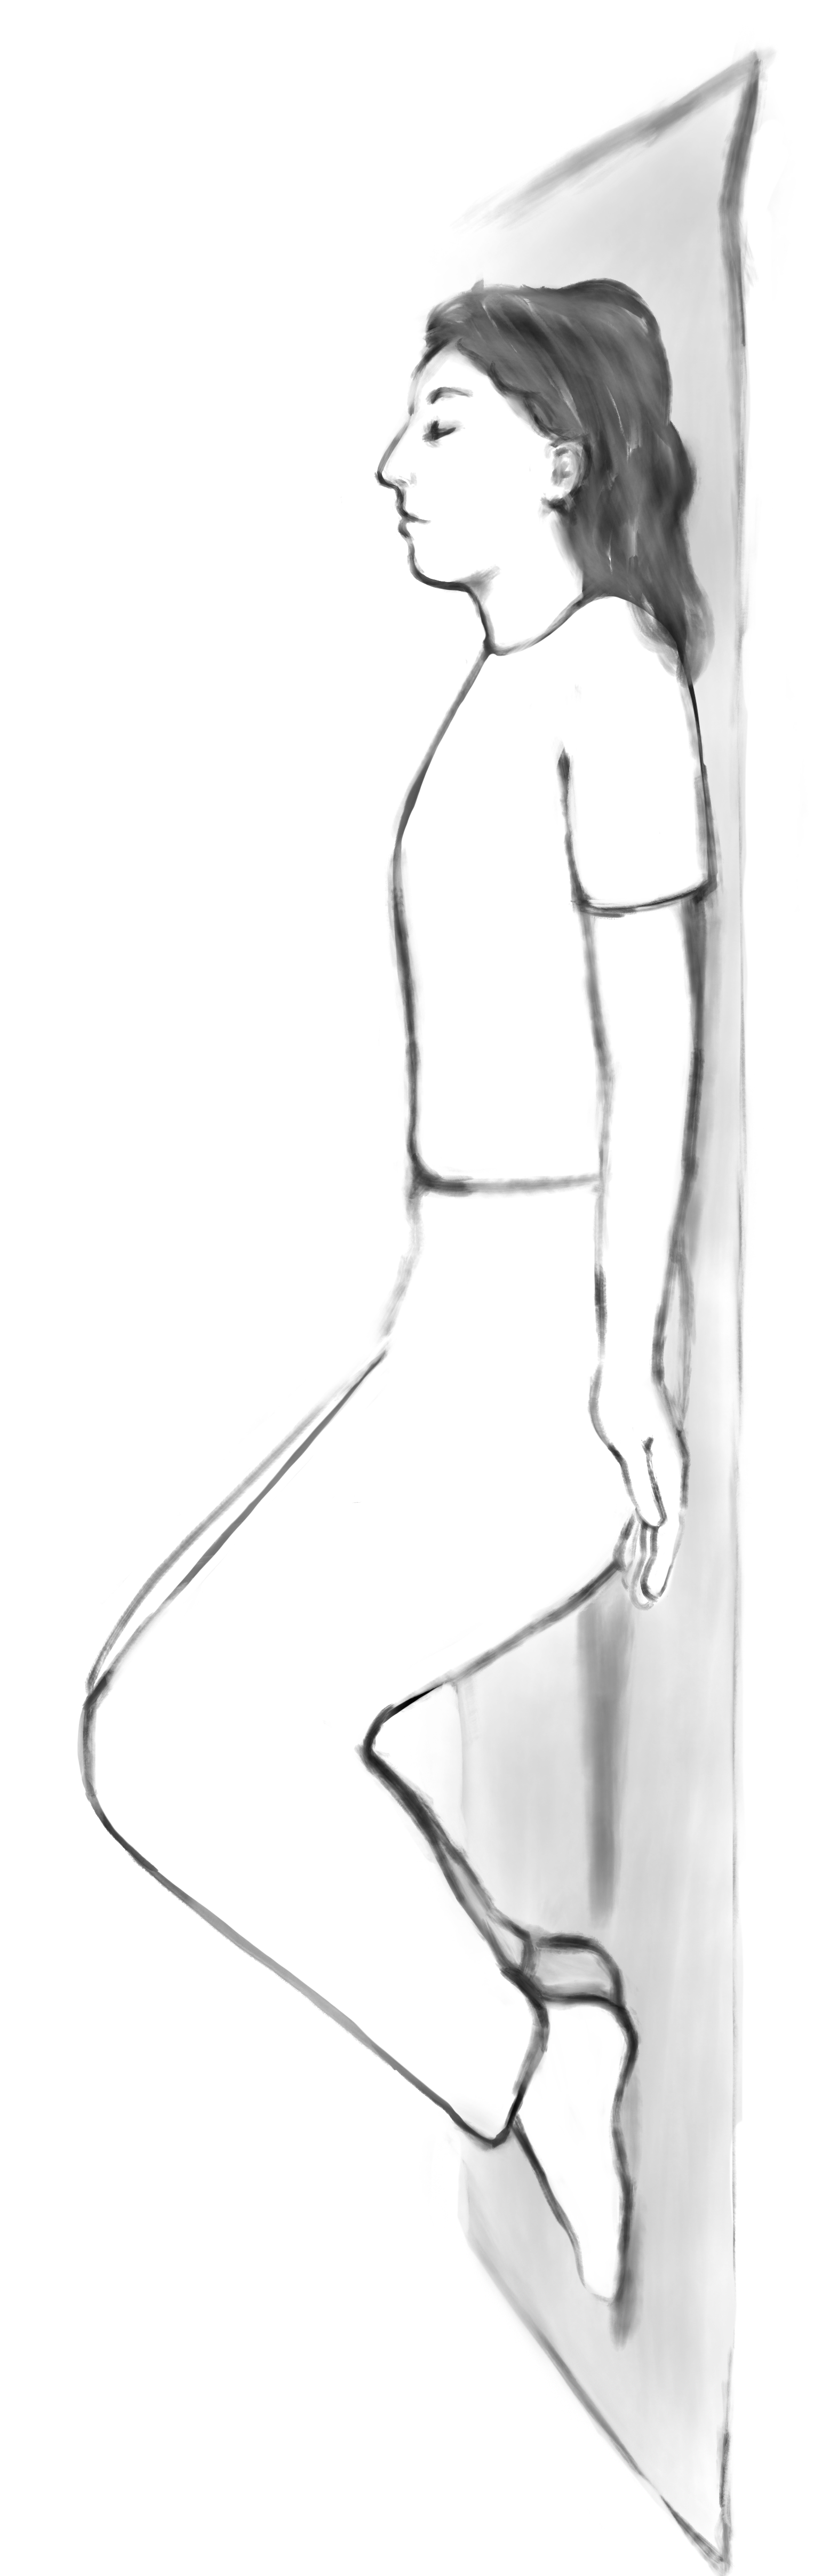
\includegraphics[height=190mm]{lying-down.png}

\illustration{Lying Down Meditation Posture}%
\label{illus-lying-down-meditation}%

\vfill\null
}
\clearpage

Before lying down, determine a clear intention to be wakeful. This sets
the suitable attitude and establishes some mental distance from our
daily activities. To further cultivate this reverential tone, we can bow
toward a Buddha shrine, and softly recite a short chant.

A yoga mat or soft carpet is useful to avoid getting sore when lying on
the hard floor. If you feel the breath becoming obstructed as the head
inclines backward, use a small pillow or a folded towel to prop up your
head. Lying down in a bed might be too soft, and it reminds the body
about sleeping.

Let the arms rest at the side of the body; if you place them on the
belly or the chest, the rising and falling movement can be distracting.
Pull up the knees, so that the feet can be flat on the mat and letting
the lower back closer to the floor. This avoids tension in the joints
and helps to maintain alertness.

Maintain this posture while relaxing the muscles in the body and
cultivate physical stillness. Direct attention inward and use the
sensation of breathing as your meditation object. Experiment with the
breath. Use it to brighten the mind and maintain clear comprehension. If
the mind drifts into dull greyness, drowsiness will follow. Setting a
timer can be useful, either to signal the end of the session, or as a
periodic reminder to remain alert.

\clearpage

\section{The effect of sounds}

\keywords{noise exposure, available cognitive capacity}

\noindent This doesn't mean that sound cannot be pleasant. Music clearly
has therapeutic effects, and can help to relax an agitated mind. It may
be \emph{very good music} (in our opinion), but how many times in a row
can we listen to it? The same single thing, when repeated over and over,
turns from pleasant to painful in a short time. Have you listened to
music for hours, but then still felt relieved when you turned it off?
`Good song, but I've been missing this silence.'

Sounds are input signals which stimulate the nervous system. Some sounds
can feel good for a while with a positive effect, while other sounds
cause irritation and distraction.

Noisy environments degrade attention and intelligence. You can probably
remember how hard it is to think clearly when there is a construction
site at your neighbour's property. Apart from anecdotal experience,
medical studies have also measured how `mental workload and visual /
auditory attention is significantly reduced'\footnote{\href{https://www.ncbi.nlm.nih.gov/pmc/articles/PMC6901841/}{The
  Effect of Noise Exposure on Cognitive Performance and Brain Activity
  Patterns (ncbi.nlm.nih.gov)}} when being exposed to noise.

\enlargethispage*{\baselineskip}

Mobile phones don't even have to make a sound to cause `brain drain'.
Another study found that `the mere presence of one's own smartphone
reduces available cognitive capacity'.\footnote{\href{https://www.journals.uchicago.edu/doi/10.1086/691462}{Brain
  Drain: The Mere Presence of One's Own Smartphone Reduces Available
  Cognitive Capacity (journals.uchicago.edu)}}

It is not surprising that traditional insight meditation retreats try to
setup a silent environment and ask participants to not bring their
mobile phones to the meditation hall, or to leave them in a locked place
for the entire retreat. Give your nervous system a break and let it
settle. Don't let it be like the crow in Santoka's haiku,\footnote{\href{https://www.goodreads.com/book/show/931086.Grass_and_Tree_Cairn}{Grass
  and Tree Cairn, Taneda Santoka}}

\begin{quote}
Cawing a crow,\\
flapping a crow,\\
with no place to settle down.
\end{quote}

\section{Chanting}

\keywords{setting a clear intention, wholesome thoughts}

\noindent At the monastery, we practise chanting before or after the
daily group meditations. First, when we arrive individually to the
Dhamma Hall, we bow three times in silence toward the Buddha shrine. The
senior monk then rings a small bell to signal the start of the chanting.
We wait in silence while he lights the candles and incense on the
shrine, and then we bow again. During the bowing, there is always
silence.

We begin the chanting together, synchronizing our voices: too soft and
we can't be heard; too loud and it's harsh; chant out of tune and we're
separated from harmony. (A good guideline is that if you don't hear your
own voice, you are chanting too softly. If you can only hear yourself,
you are too loud.) The text of the chants are recollections of the
Buddha and his teachings. This is a practice of directing the mind
toward wholesome thoughts. This ordered, symbolic ceremony uses a rhythm
of speech and action as a skilful tool to clear the mind before the
silence of meditation.

The exact routine varies between monasteries. The morning meditation at
Sumedhārāma in Portugal starts at 5am. We start with an hour of sitting
meditation, during which there is no speaking or chanting. When you
enter, there is silence -- a shared space for inner reflection. At the
end of the meditation the senior monk rings a bell and this is followed
by 15-20 minutes of chanting.

\section{Boredom}

\keywords{boredom, learning about the mind, inner peace, sense-restraint}

\noindent `Doesn't it get boring?' From time to time, a school will
bring a whole class of children to the monastery to meditate in silence
(perhaps hoping that they will become more quiet afterward). Most
likely, the majority of them feel terribly bored. They have no interest
to be there from the outset. But children are clever and they often
learn that they will escape sooner if they tolerate the strange ideas of
adults.

When our regular visitors come to meditate, their relationship to this
mental state is different from the outset. They come with an interest in
learning about themselves and their mind. When you look closer at it,
the `boring' can become rather interesting. Boredom changes as soon as
you look at it. `Not much is happening, just the breathing. Is that a
problem for me? Am I creating that problem? Can I stop creating such
problems for myself? Sitting here and breathing is actually a pleasant
feeling.'

When practising mindfulness of breathing, there is a gladness born of
sense restraint. The mind relaxes, and the thinking can be allowed to
stop. We are silently observing experience and there is no need to
comment.

Boredom is a combination of factors: the desire for excitement and
novelty, active dismissal of the present, and the attitude that we
already know what is going to happen. Is it not intrinsic to the
situation, but a habit of the untrained and restless mind.

The Buddha compared restlessness to how an elephant feels when the
trainer first restrains him by tying him to a strong post. The elephant
is unfit to train while he still longs to wander in the wilderness as he
wishes. A good trainer gradually restrains the restless elephant, until
they learn to remain content.\footnote{\href{https://suttacentral.net/mn125}{MN
  125}, The Level of the Tamed} In the sutta, Prince Jayasena, who lives
in a palace surrounded by distractions, doesn't even believe that inner
peace is possible through sense-restraint, since he has never
experienced such peace himself.

\enlargethispage*{\baselineskip}

In the meditation hall the door is open, you can stand up and walk out
any time. But you are there because you have felt that the untrained
mind keeps making painful mistakes and causes trouble for itself and
others. If you walk a thousand steps in a thousand directions, you will
just get tired and angry that you didn't get anywhere. It is good to
recognize the need to be the trainer of our restless mind. We learn what
the right direction is and keep making steps in that direction.

\begin{quote}
For the mind that is difficult to subdue,\\
flighty, flitting wherever it will,\\
restraint is good,\\
a restrained mind brings happiness.

\bigskip

\quoteRef{%

Dhp 35.\footnote{\href{https://www.ancient-buddhist-texts.net/English-Texts/Dhamma-Verses/03-Mind.htm}{Dhammapada,
  translated by Ānandajoti Bhikkhu}}

}
\end{quote}

\section{Shrine}

\keywords{creating sacred spaces, symbolism of a Buddha shrine}

\noindent I didn't always create a Buddha shrine in the room or hut
where I stayed at the monastery. In the beginning, I thought they were
part of conforming to institutional expectations. So I mostly ignored
and subtly resented pictures and statues. I felt other people expected
me to venerate them, and with a contrary attitude, I wasn't going to do
what (I thought) they expected.

My reaction was like that of the school kids: I was clever enough to
tolerate the symbols and arrogant enough to think I already knew what
they meant. Believing oneself clever makes one feel superficially
dismissive and bored with everything. It is a self-stupefying
combination. Thinking that \emph{I know} closes our mind, so we can't
find out that, in fact, we don't know. The British psychologist Iain
McGilchrist compares this to being stuck in a labyrinth of
mirrors:\footnote{\href{https://www.goodreads.com/book/show/6968772-the-master-and-his-emissary}{The
  Master and His Emissary: The Divided Brain and the Making of the
  Western World by Iain McGilchrist}} all you can see is what you tell
yourself, and you'll never find a way out.

A small crack must have appeared on those mirrors, because eventually I
picked up that nobody was making such expectations of me. I was creating
both sides of the story and I felt consumed over something I only
imagined.

Making a Buddha shrine opens up a small space in the place we live, a
reminder to stop the hurry and make space for awakening. The Buddha
shrine in the meditation hall gives us the same message through silence.
A personal shrine is a gift for ourselves from ourselves. It is not for
answering other people's expectations, or even for the Buddha. The
historical Buddha passed away 2600 years ago and is beyond expecting or
needing anything from us. Other people have enough to worry about and
don't think about us as much as we assume.

I remember thinking, `Why don't I have space for the Buddha in the place
where I live?' Then I started to cut some wood planks and made a small
shelf for the shrine. Buddha shrines are often quite plain: one or more
Buddha figures, candles, incense and flowers. The Buddha represents
awakened consciousness in the human form. The candles are for wisdom
which makes things visible, as light in darkness. The incense can remind
us when the Buddha spoke about virtue, `the fragrance of virtue pervades
all directions' (Dhp 54). The flowers are a symbol of virtue, happiness
and impermanence. They are like our practice: they bring happiness if we
take good care of them and renew them frequently; while their fading is
a reminder of transience.

I offer these words of reflection with the intention that they may
encourage your practice. The teacher is the Buddha, the source of
illuminating explanations leads back to him. I am grateful that his
teachings have been carried on through the centuries by each generation
up to this day. Let's use them to turn the noisy confusion of the mind
into understanding silence.
